\section{Circuito analógico de entrada\label{testcircuito}}

Aunque montaje del módulo de entrada ha surgido únicamente de la curiosidad académica y no de conveniencia técnica, se van a realizar una serie de medidas que permitan caracterizar su funcionamiento básico.

\subsection{Saturación y dependencia con la frecuencia}
Es necesario tener en cuenta que para realizar todas las medidas que se presentan a continuación ha sido necesario generar dos señales de entrada para el circuito. No hay que olvidar que al tratarse de una entrada balanceada, se debe introducir una señal en un canal y duplicarla en contrafase en el otro canal de entrada. Afortunadamente, el generador de funciones disponible en el laboratorio ofrece esta posibilidad únicamente pulsando un botón. En lo sucesivo, cuando me refiero a la señal de entrada siempre me referiré al conjunto de la señal en cuestión más el duplicado en contrafase.

En este apartado se pretende caracterizar la respuesta del circuito frente a entradas de diferentes tensiones, utilizando diferentes posiciones del potenciómetro y permitiendo hallar el punto de saturación del conjunto para una entrada sinusoidal. Las medidas tomadas son las mostradas en la tabla siguiente.\\

\begin{table}[htb]
\centering
\begin{tabular}{|c |c |c |c |c |c|}
%%%%%%%%%%%%%%%%%%%%%%%%%%%%%%%%%%%%%%%%%%%%%%%%%%%%%%%%%%%%%%%%%%%%%%%%%%%%%%%%%%%%%%%%%%%%%%%%%%%%%%%%%%%%%%%
\hline
$V_{in}(mV)$            &$Pos.~Pot.$   &$V_{out}(mV)$          &$~~~~G (V/V)~~~~$      &$~~G (dB)~~$     &$Rango~Pot.(dB)$   \\
\hline
\multirow{2}{1.5cm}{\centering{518,8}} & Min. & 365,6 &  0.7047 & -3,04 & \multirow{2}{1.5cm}{\centering{8,12}} \\
                                      & Max. & 931,3 &  1,7951 & 5,08 &                                       \\ \hline
\multirow{2}{1.5cm}{\centering{1018}} & Min. & 643,8 &  0,6319 & -3,99 & \multirow{2}{1.5cm}{\centering{12,05}} \\
                                      & Max. & 2578 &  2,5304 & 8,06 &                                       \\ \hline
\multirow{2}{1.5cm}{\centering{2016}} & Min. & 1243 &  0,6170 & -4,19 & \multirow{2}{1.5cm}{\centering{9,10}} \\
                                      & Max. & 3547 &  1,7594 & 4,91 &                                       \\ \hline
\multirow{2}{1.5cm}{\centering{3313}} & Min. & 1875 &  0,5660 & -4,94 & \multirow{2}{1.5cm}{\centering{9.59}} \\
                                      & Max. & 5656 &  1,7072 & 4,65 &                                       \\ \hline           
\end{tabular}
%\caption{\label{tabla:sat_medidas}Relación de tiempo de trabajo destinado a cada ámbito.}
\end{table}

En esta tabla, la columna \emph{Pos. Pot} hace referencia la posición del potenciómetro, es decir, si estaba ajustado al mínimo o al máximo, lo que permite estimar el rango de la ganancia en la columna \emph{Rango. Pot}. Se puede apreciar como la mayor sensibilidad se obtiene para la entrada de $1V_{pp}$ aproximadamente. La última medida corresponde al punto de saturación, el cual se ha obtenido empíricamente aumentando la tensión de entrada hasta que se observase recorte en la salida (con ganancia máxima), el proceso se muestra en la figura \ref{fig:medsat}.

\begin{figure}[!hbt]
\begin{center}
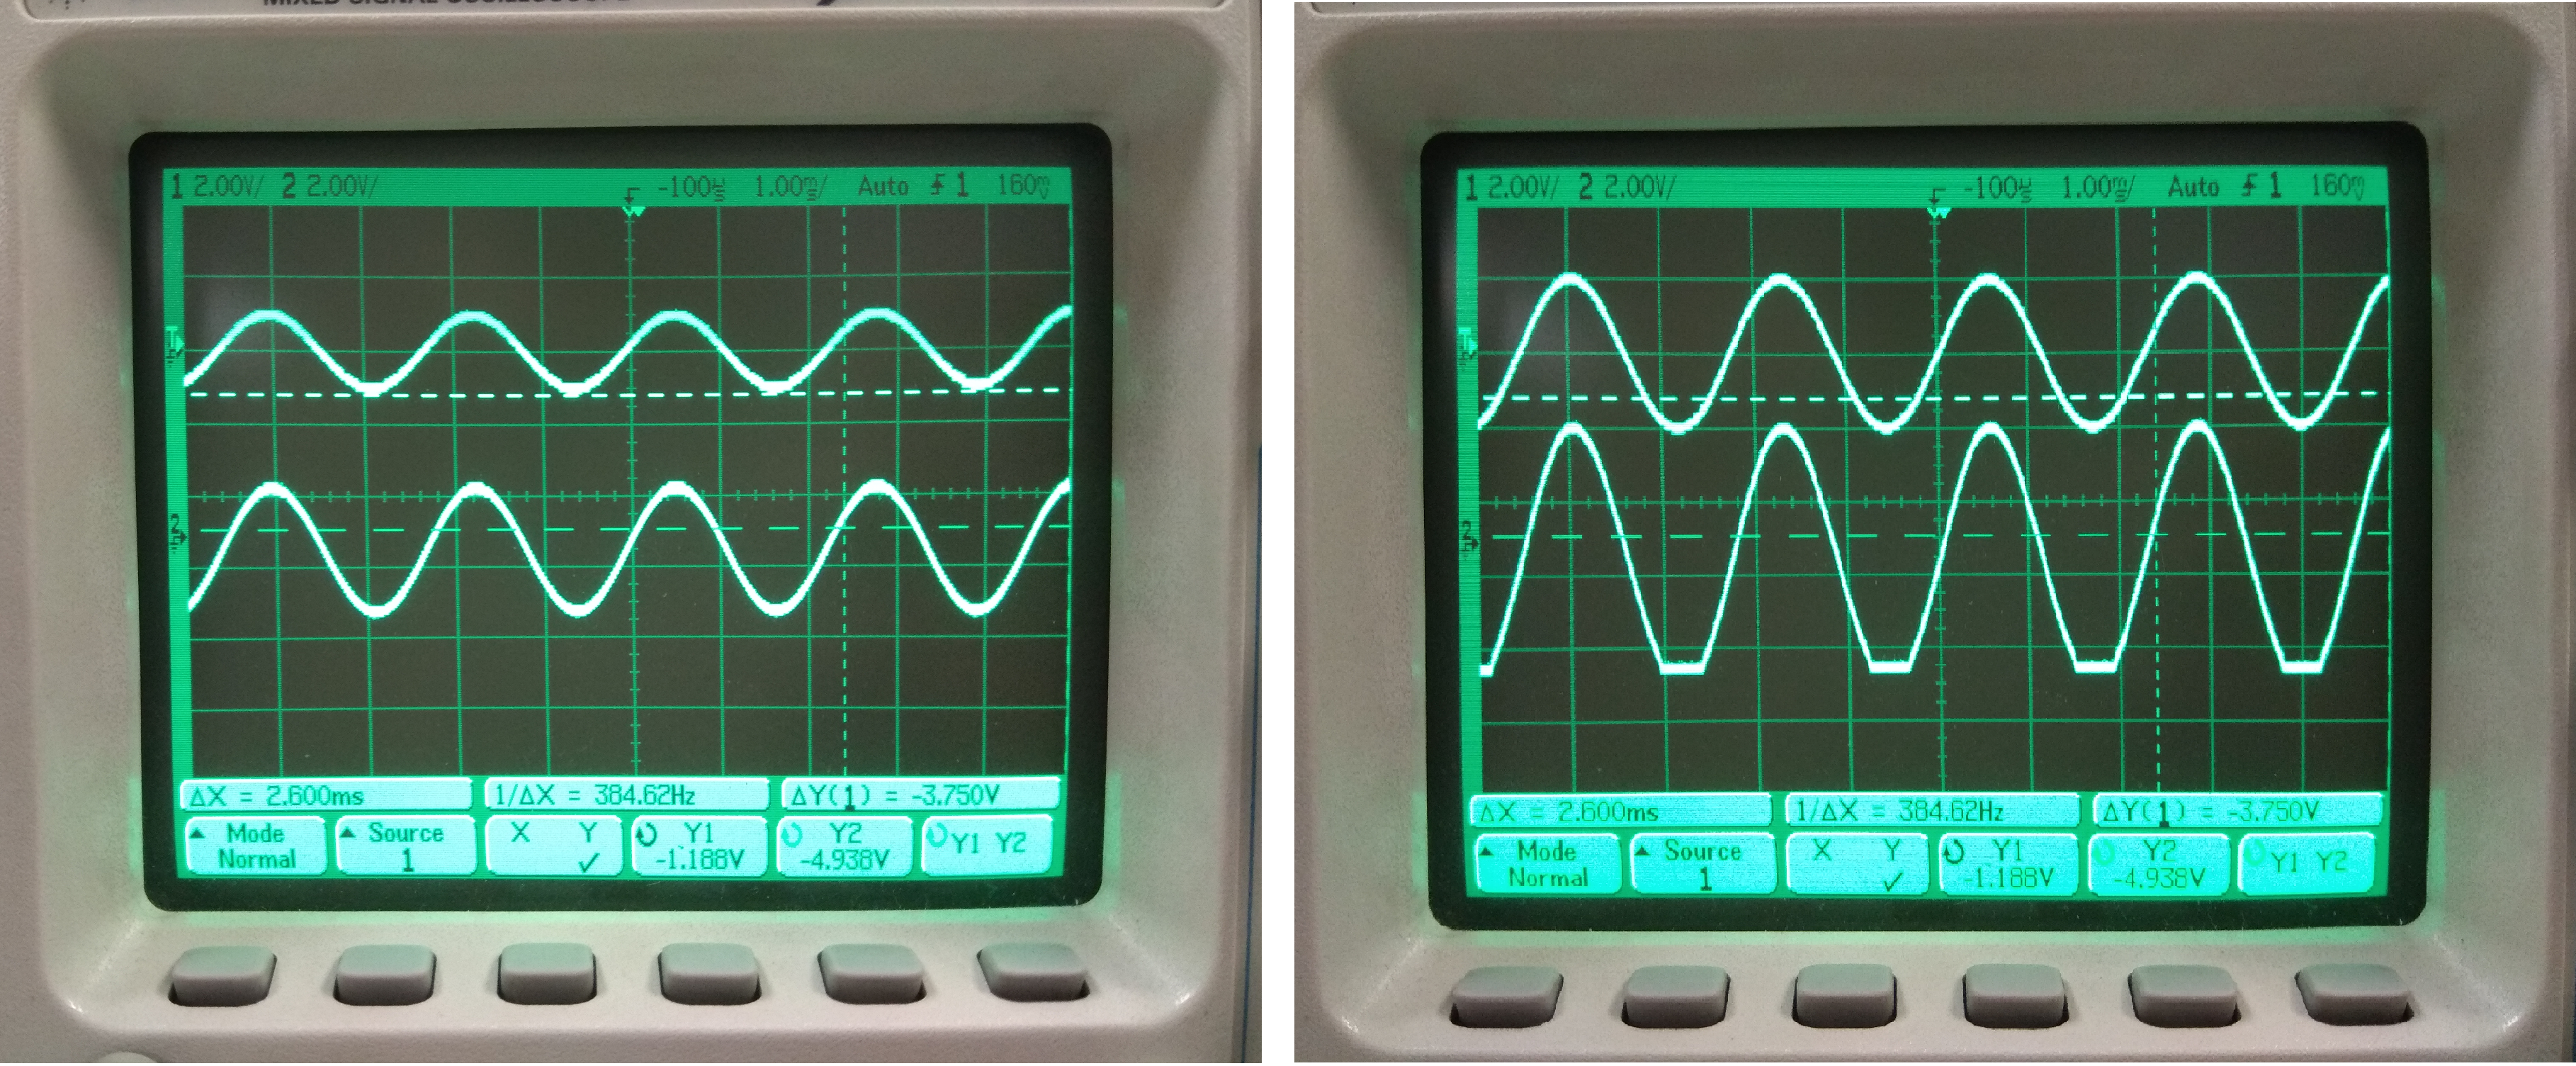
\includegraphics[width=12cm]{img/medsat.png}
\caption{\label{fig:medsat}Fotografías de las medidas realizadas buscando el punto de saturación}
\end{center}
\end{figure}

\subsection{Dependencia de la ganancia con la frecuencia}

Para poder verificar un buen comportamiento del circuito en todo el espectro, se ha introducido en la entrada una señal de $1~V_{pp}$ modificando el valor de la frecuencia. El resultado se ha graficado en la figura \ref{fig:medfreq} añadiendo una ventana amarilla que expresa el umbral del oído humano. Para tomar las medidas se han priorizado las frecuencias fundamentales de las notas del saxofón, tal y como se detalla en el Apéndice \ref{ap:datosmedidasfreq}.

\begin{figure}[!hbt]
\begin{center}
\includegraphics[width=14cm]{img/relaciongf.png}
\caption{\label{fig:medfreq}Dependencia de la ganancia con la frecuencia}
\end{center}
\end{figure}

Estas gráficas (izquierda en unidades lineales y decibelios en la derecha) resultan un poco engañosas debido a que los valores de los ejes están muy detallados: la línea roja discontinua marca el ancho de banda a $-3~dB$. Se puede observar como se produce una caída esperada de la ganancia conforme aumenta la frecuencia, sin embargo, en el espectro audible es prácticamente nula. La consecuencia de ello es que se obtiene un ancho de banda con un margen más que suficiente para captar todos los sonidos provenientes del instrumento. 

En la fuente bibliográfica utilizada \cite{Preamp} se detallan parámetros adicionales que permiten caracterizar el circuito de forma más precisa. Dado que el circuito funciona correctamente, no he considerado necesario incluir un banco de pruebas más exhaustivo.

\section{Algoritmo de \emph{Vocoder de fase}}

Para probar el algoritmo que se va a implementar se ha utilizado un fragmento breve interpretado con saxofón alto del tema \emph{Billie's Bounce} de \emph{Charlie Parker}. La grabación de este fragmento está realizada con un micrófono corriente no profesional y se ha guardado en formato \emph{.wav}, es decir, sin compresión. Este formato, al igual que Matlab, utiliza una frecuencia de muestro $F_{s} = 44.1~kHz$.

El fichero de prueba se encuentra en el Apéndice \ref{ap:pruebaalgoritmo}. Esta función precisa de una ruta de archivo de audio que se va a octavar y de un entero que se corresponde con un cierto número de muestras de retraso. Este último parámetro permite cuantificar los efectos de la latencia en la FPGA.

\begin{figure}[hbt]
\begin{center}
\includegraphics[width=15cm]{img/testAlFreq.png}
\caption{\label{fig:testFreq}Suma de las componentes en frecuencia}
\end{center}
\end{figure}

El resultado de la prueba son dos archivos de audio: uno contiene el fichero de entrada octavado y el otro mezcla la entrada con el fichero octavado en una proporción de 35\% y 65\% respectivamente. Lógicamente, es en este último en el que la latencia tiene efecto. Adicionalmente se ha graficado tanto la suma de las componentes en frecuencia (figura~\ref{fig:testFreq}) como en el dominio del tiempo (figura~\ref{fig:testTime}) ambos con latencia nula. En la primera podemos observar claramente como los picos se encuentran en frecuencias de la mitad de valor debido a la octavación. Aunque pueda parecer que el resultado muestra la serie armónica, hay que recordar que en este fragmento se han interpretado múltiples notas, cada una con sus correspondientes frecuencias y armónicos asociados, por lo que la similitud que vemos entre esta gráfica y la serie armónica se debe a que las notas de la serie se utilizan más frecuentemente en la melodía. 

\begin{figure}[!bht]
\begin{center}
\includegraphics[width=15cm]{img/testAlTime.png}
\caption{\label{fig:testTime}Comparativa de los ficheros resultantes}
\end{center}
\end{figure}

En la gráfica correspondiente al dominio del tiempo se observa una ligera pérdida de amplitud en la señal debido al procesado. Para cuantificar el valor de estas pérdidas se utiliza el cociente entre el valor medio de la señal de salida entre el de la entrada, resultando en \textbf{1,5586 dB} para la señal octavada y \textbf{2,3890 dB} para la mezcla de ambas. También se puede apreciar como la forma de onda no se ha distorsionado en exceso; la calidad del audio resultante resulta razonablemente buena teniendo en cuenta que se ha pretendido simular el comportamiento de la FPGA con una longitud de transformada de 512 muestras de 16 bit, valores que distan de lo que las fuentes bibliográficas consideran como admisible en término de calidad.

\section{Sobre la implementación en FPGA}

Sin lugar a dudas, el parámetro más importante del sistema es la latencia. No obstante, debido a que no se ha podido finalizar completamente la implementación de todo el algoritmo habrá que conformarse con realizar una estimación. Esta deberá ser lo más realista posible para poder comparar el diseño de la arquitectura con otros existentes en la literatura.

La cifra conocida de la latencia derivada del montaje de las tramas y las ventanas\footnote{En este caso se utilizan las palabras trama y ventana de forma equivalente en referencia a las agrupaciones de 512 muestras que serán procesadas en conjunto.} se obtiene prácticamente de forma inmediata: el tiempo que se emplea en rellenar una ventana es la longitud de la ventana multiplicada por la velocidad a la que se llena, el periodo de muestreo $t_{s}$. Así obtenemos un valor de $512 \cdot (512 \cdot 2)/(50\cdot10^{6})  = 0.010~s \equiv 10,48~ms$. No obstante, esta cifra es engañosa debido a que no se espera a que se lea la trama completa para empezar la operativa de la FFT. Como esta se empieza a cargar justo cuando entra la muestra 256, es decir, en la mitad de la trama, se comienza el procesado de la FFT justo después de que se cargue la última muestra de la misma. En consecuencia, no hay que contar el tiempo de volcado desde la memoria hacia el módulo que realiza la FFT.

Debido a que el módulo FFT e iFFT son iguales, la latencia que añaden al sistema es idéntica. Vivado proporciona una medida de esta latencia de 1652 ciclos, que operando a $100~MHz$ equivalen a $16,52~\mu s$. La operativa de la FFT comienza un ciclo de bit más tarde de la carga del último dato por la construcción de la máquina de estados, por lo que hay que sumarlo al total posteriormente.

Una vez en el dominio transformado, según el diagrama del algoritmo previamente descrito en el apartado \ref{calc_alg}, el siguiente paso es obtener sus componentes en forma polar, pudiéndose realizar empleando los módulos CORDIC de Vivado \cite{cordicdoc}. Estos módulos emplean 20 ciclos para realizar las operaciones. 

\begin{figure}[!bht]
\begin{center}
\includegraphics[width=15cm]{img/estimacionlat.png}
\caption{\label{fig:estlat}Diagrama del tiempo de carga de 8 ventanas}
\end{center}
\end{figure}

Llegado a este punto es razonable afirmar que la latencia introducida durante el procesado resulta despreciable frente a la que introduce el montaje de las tramas. Aún así, se va a utilizar un valor de $0,7~ms$ para cuantificar el tiempo de procesado. Este valor es muy pesimista, teniendo en cuenta los 20 ciclos que emplean los CORDIC, el tiempo de carga de la iFFT (esta vez a $100~MHz \rightarrow 512\cdot1/100\cdot10^{6} = 5,12~\mu s$) y la latencia de la misma, difícilmente se van a superar los $700~\mu s$ elegidos.

\begin{figure}[thb]
\begin{center}
\includegraphics[width=14cm]{img/efectolatencia.png}
\caption{\label{fig:efectolatencia}Efecto de la latencia en la forma de onda}
\end{center}
\end{figure}

Finalmente se va a estimar la latencia del sistema sumando a los $700~\mu s$ descritos el tiempo de espera tras 8 ventanas el cual, según la figura \ref{fig:estlat}, será de 1408 tramas a la frecuencia de muestreo resultando en un valor total de latencia de $1/F_{s} \cdot 1408 + 700 \cdot 10^{-6}=29,53~ms \approx 30~ms$. 

Para simular el efecto que tendría en el oído se ha utilizado el desfase artificial introducido en el código de Matlab previamente descrito. Como el código entiende la latencia en forma de un número de muestras retrasadas, se ha calculado el valor del mismo en base a la frecuencia de muestreo de Matlab: $44,1~kHz$. Así, $30 \cdot 10^{-3}/F_{s-MATLAB}=1323$. En la figura \ref{fig:efectolatencia} se puede apreciar el efecto de la latencia en la forma de onda de la salida: en la primera gráfica se muestra la entrada, en la del medio la salida con el valor de latencia obtenido en el cálculo previo y en la última se fuerza una latencia elevada para que resulte apreciable. Los resultados se han guardado en archivos de audio para su comparación.

\subsection{Uso de recursos y conclusiones}

Tras comentar el tiempo que se emplea para realizar el algoritmo se adjuntan en la figura \ref{fig:estarea} las estadísticas sobre la carga computacional para llevar a cabo el algoritmo descrito. 

\begin{figure}[!bht]
\begin{center}
\includegraphics[width=15cm]{img/areafpga.png}
\caption{\label{fig:estarea}Disponibilidad de recursos de la FPGA según Vivado}
\end{center}
\end{figure}

Los datos obtenidos en la figura \ref{fig:estarea} se corresponden únicamente con la parte del algoritmo que se ha implementado. Adicionalmente, se han añadido los módulos CORDIC que serían necesarios para mejorar la precisión de los datos. En cualquier caso, es evidente que la FPGA no requiere de muchos de sus recursos para poder implementar el código descrito, habiendo un amplio margen de carga. Además hay que tener en cuenta que durante el desarrollo de la implementación siempre \textbf{se ha priorizado latencia frente a consumo de recursos}, de forma que se ejecute el código en un tiempo de respuesta razonable.

Una vez realizadas estas mediciones se puede concluir que \textbf{la latencia no es un punto crítico a la hora de implementar sistemas de procesado de audio en tiempo real en FPGA} en comparación con otras tecnologías extendidas en el mercado profesional, como la electrónica analógica o el uso de circuitos integrados y microprocesadores. La latencia ha resultado mínima teniendo en cuenta que todavía hay margen de mejora de la misma. 

Si no existen sistemas profesionales de audio desarrollados con estas tecnologías es debido al \textbf{alto coste de diseño} que es necesario para implementar el sistema y al \textbf{alto coste de producción} frente a un microprocesador, por ejemplo. Sin embargo, aquí entran en juego otras ventajas de la FPGA como su flexibilidad frente a cambios y su robustez. La etapa analógica resulta insustituible independientemente de la tecnología de procesado utilizada después debido a que siempre será necesario adecuar la señal y amplificarla.